\chapter{Introducción General}

\label{Chapter1} % \ref{Chapter1} 
\label{IntroGeneral}

%-------------------------------------------------------------------------------

\newcommand{\keyword}[1]{\textbf{#1}}
\newcommand{\tabhead}[1]{\textbf{#1}}
\newcommand{\code}[1]{\texttt{#1}}
\newcommand{\file}[1]{\texttt{\bfseries#1}}
\newcommand{\option}[1]{\texttt{\itshape#1}}
\newcommand{\grados}{$^{\circ}$}

%-------------------------------------------------------------------------------

En este capítulo se presentan la necesidades generales de la industria, y las particulares del cliente que se pretenden satisfacer. Adicionalmente, se provee de una introducción técnica superficial de las tecnologías involucradas.

\section{Motivación}
\label{motivacion}

	\subsection{Necesidades generales}

		\subsubsection{Progreso tecnológico}

			La producción de bienes y servicios experimentó una serie de innovaciones, que fueron reemplazando distintas habilidades y características del hombre. Se identifican cuatro hitos en este proceso, los cuales se denominan revoluciones industriales.
		
			La primer revolución industrial consistió en reemplazar las fuerzas físicas de hombres y bestias, en favor de nuevas fuentes de energía para obtener trabajo. Vapor, combustión, electricidad, ect. 

			La segunda revolución industrial hizo obsoleta la capacidad de polivalencia de los humanos al crear líneas de montaje, gracias a Henry Ford nació la organización productiva moderna.

			Un tercer hito fue la llegada de la electrónica y ordenadores que permitió crear nuevas tecnologías de instrumentación y control, esto permitió reemplazar la motricidad gruesa y fina de las personas, y también desplazó las tareas manuales de control de actuadores. 

			Finalmente, la cuarta y actual revolución industrial consiste en superar las capacidades cognitivas biológicas, al conectar los dispositivos entre sí y con ordenadores que proveen persistencia en las mediciones, y su análisis a través de la inteligencia artificial.
	
		\subsubsection{Modernización}

			Las plantas de producción que se encuentran en la República Argentina están retrasadas en su progreso tecnológico, la mayoría no ha incorporado sistemas electrónicos en sus procesos o productos. Esto plantea la necesidad de crear un sistema que logre adaptar la antigua tecnología existente, y que permita integrarla a los nuevos paradigmas de trabajo. Finalmente, la actual situación tecnológica, se traduce en la demanda de un sistema que permita unir capital viejo y sus protocolos antiguos, con las nuevas posibilidades que ofrece la cuarta revolución industrial.

		\subsubsection{Comercio internacional}
			
			El avance tecnológico produce cambios en el marco normativo de las naciones, la consecuencia es la necesidad de conformar con requisitos mínimos de capital, para cumplir con los requerimientos jurídicos necesarios para ingresar dentro de nuevos mercados. El retraso tecnológico ya no solo genera una pérdida de competitividad, sino que también implica una barrera legal que impide que las empresas dentro de la jurisdicción argentina, coloquen sus mercancías en otras latitudes. Por incumplimiento en normas que apuntan a la calidad de la producción o a la protección del medio ambiente.

			Las necesidades generales expuestas promovieron el interés de crear un proyecto que permita asistir a las empresas en su incorporación a la cuarta revolución industrial. Si las compañías argentinas no lo lograran, probablemente queden fuera del mercado mundial en pocos años.

	\subsection{Necesidades del cliente}
	
		\subsubsection{Gador S.A}
		
			\emph{Gador S.A} es una compañía cuya misión es \emph{producir medicamentos para la salud humana, con la mejor calidad disponible, y ponerlos al alcance de la comunidad a precios accesibles}. 

			La arquitectura de monitoreo ambiental dentro de sus plantas se encuentra gestionada por el producto \emph{Enterprise Buildings Integrator (EBI)}, de la empresa \emph{Honeywell}. Esta solución propietaria, fue adquirida con una licencia \emph{modbus universal} y permite comunicarse desde los dispositivos en campo, utilizando solo el \emph{fieldbus} mencionado.

			Hay en planta una serie de \emph{Controladores Lógicos Programables (PLC)} que cumplen la función de ser puntos de agregación para la red de sensores que se encuentra en cada cuarto. El instrumental se comunica con su respectivo \emph{PLC}, a través de protocolos cableados, como pueden ser \emph{4-20mA} y \emph{Digital in/out}. La red que une el servidor \emph{EBI} con los \emph{PLCs} es \emph{Modbus TCP}, como se visualiza en la figura \ref{fig:redGador}.
			
			\begin{figure}[h]
				\centering
				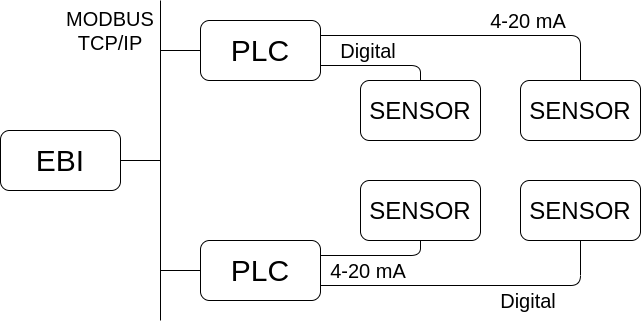
\includegraphics[width=\textwidth]{./Figures/chapter1/redGador.png}
				\caption{Red industrial actual en Gador.}
				\label{fig:redGador}
			\end{figure}
		
		\subsubsection{Marco normativo}
		
			Para acceder al mercado de los Estados Unidos de Norte América, se deben satisfacer los requerimientos del \emph{Code of Federal Regulations - Title 21 - Food and Drugs Chapter - Part 11 (21CFR11)}. Esta es la principal razón para utilizar el sistema \emph{EBI}, ya que el producto se encuentra aprobado por la \emph{FDA}, por lo tanto, es indispensable que este ambiente de producción continúe operando aún cuando los protocolos que utiliza son antiguos.
			
			El primer problema que se puede observar es el acarreo de tecnologías \emph{legacy} en aras de satisfacer las normas que permiten el comercio internacional, sin incurrir en mayores erogaciones al invertir en un nuevo sistema que se encuentre aprobado por la \emph{FDA}.

		\subsubsection{Metrología}
		
			La mediciones reportadas por los sensores deben ser significativas, eso solo puede ser logrado si el instrumental es sometido a un plan de calibración y a una reubicación periódica según estudios de mapeo térmico, que determinan los puntos críticos del volumen a medir.
			Las recurrentes migraciones de sensores provocan costosos procesos de certificación de cableados, surge de esta situación la necesidad de utilizar modernos protocolos de comunicación inalámbrica que permitan alcanzar un consumo energético lo suficientemente bajo, para que las baterías de los sensores duren como mínimo un año.
			
			Los estudios de mapeo térmicos obtienen los puntos críticos del volumen del ambiente, estos puntos críticos son las posiciones que los sensores deben ocupar.
			
			Se necesita disponer de una gestión de sensores, cuyo nivel de sofisticación deseado no es satisfecho por los \emph{PLCs}, se manifiesta entonces la necesidad de desarrollar un sistema que gestione puntos de agregación y sensores de mayor complejidad, este objetivo nace de los costosos procesos de calidad que disparan la incorrecta administración de los dispositivos, cuando estos impactan en la base de datos de \emph{EBI} con valores erróneos.		

\section{Introducción técnica}
\label{introTecnica}

\section{Estado del arte}
\label{estadoArte}

\section{Objetivos y alcance}
\label{objetivos}
